\documentclass[10pt]{report}
\usepackage[utf8]{inputenc}
\usepackage[italian]{babel}
\usepackage{multicol}
\usepackage[bookmarks]{hyperref}
\usepackage[a4paper, total={18cm, 25cm}]{geometry}
\usepackage{graphicx}
\usepackage{xcolor}
\usepackage{textcomp}
\graphicspath{ {./img/} }
\usepackage{listings}
\usepackage{makecell}
\lstdefinestyle{customasm}{
  belowcaptionskip=1\baselineskip,
  frame=line,
  xleftmargin=\parindent,
  language=[x86masm]Assembler,
  basicstyle=\ttfamily,
  commentstyle=\itshape\color{purple!40!black},
}
\lstset{escapechar=@,style=customasm}
\lstnewenvironment{C}
  {\lstset{language=C++,frame=none}}
  {}
\begin{document}
\title{Artificial Intelligence Fundamentals}
\author{Federico Matteoni}
\date{A.A. 2021/22}
\renewcommand*\contentsname{Index}

\maketitle
\begin{multicols}{2}
\tableofcontents
\end{multicols}
\pagebreak
\section{Introduction}
Prof.s: Maria Simi, Vincenzo Lomonaco\\
AI is taking over the world. Formalizing common sense is a lot more difficult. We can formalize knowledge in very specific and small domains. But is deep learning the final solution to AI? "It will transform many industries, but it's not magic. Almost all of AI's recent progress is based on one type of AI, in which some input is used to quickly generate simple response." (\textit{Andrew Ng})\\
\textit{This} AI can do supervised learning, but requires huge amount of data (tens of thousands of pictures to build a photo tagger, for example). The rule of thumb of Ng is: if a person can do a mental task with less than one second of thought, we can automate it using AI either now or in the near future.\\
The challenges are:
\begin{list}{}{}
	\item Software is not a problem, the community is open and the software can be replicated the software can be replicated
	\item Data is exceedingly difficult to get access to. Data is the defensible barrier for many businesses
	\item Talent, because downloading and applying open-source software to your data won't work. AI needs to be customized to context and data, that's why there's a war for the scarce AI talent that can do this work.
	\item Computational resources are also very important.
\end{list}
\paragraph{Deep Learning} Is only one approach inside the much wider field of ML and ML is only one approach in the wider field of AI. Book: \textit{Thinking Fast and Slow}, Kahneman. Two systems: system 1 does perceptual tasks, simple computations, system 2 instead does complex computation, recalling from memory\ldots this is a distinction in our brains.
\paragraph{Machine Learning} Is AI all about machine learning? Possible arguments against ML are:
\begin{list}{}{}
	\item Explanation and accountability: ML systems are not (yet?) able to justify in human terms their results. For some applications this is essential: knowledge must be meaningful to humans to be able to generate explanations? Some regulations requires the right to an explanation in decision-making, and seek to prevent discrimination based on race, opinions, sex\ldots (see GDPR)
	\item ML systems learn what's in the data, \textbf{without understanding what's true or false, real or imaginary, fair or unfair}. It is possible to develop unfair, bad models. People are generally more critical about information.
\end{list}
Building AI systems is a goal far from being solved, still quite challenging. Complex AI systems requires the combination of several techniques and approaches, not only ML.
\paragraph{AI Fundamentals} Is mostly about reasoning and \textit{slow thinking}. Different approaches, "good old-fashioned artificial intelligence" or "symbolic AI": teaching about the foundations of the discipline, now 60 years old.
\paragraph{Symbolic AI} High-level human readable representations of problems, the general paradigm of searching for a solution, knowledge representation and reasoning, planning. Dominant paradigm from the mid 1950s until late 1980s.\\
Central to the building of AI systems is the physical symbol systems hypothesis (PSSH), formulated by Newell and Simon (\textit{Computer Science as Empirical Inquiry: Symbols and Search})\\
The approach is based on the assumption that many aspects of intelligence can be achieved by the manipulation of symbols (the PSSH): \textit{a physical symbol system has the necessary and sufficient means for general intelligent action}.\\
Human thinking is a king of symbol manipulation system (so a symbol system is \textbf{necessary} for intelligence), and machine can be intelligent (a symbol system is \textbf{sufficient} for intelligence). This cannot be prove, we can only collect empirical evidence: observation and experiments on human behavior in tasks requiring intelligence, and solving tasks of increasing complexity.
\paragraph{Strong and Weak AI} The Chinese room argument, by John Searle, introduced the following distinction: strong ai relies on the \textit{strong} assumption that human intelligence can be reproduced in all its aspects (general AI), including adaptivity, learning, consciousness\ldots, while weak AI is the simulation of human-like behavior, without effetctive thinking or understanding, no claim that it works like the human mind. Dominant approach today, fragmented AI.\\
One strong argument against strong AI is the lack of needs by the systems: biological need, safety, relationships, self esteem, self-actualization (Maslow's hierarchy of needs).\\
\textit{What stands in the way of all-powerful AI is not a lack of smarts: it's that computers can't have needs, cravings or desires.}\\\\
\textbf{AI is the enterprise of building intelligent computational agents}
\paragraph{Agents} An agent is something that acts in an environment. We are interested in what an agetn does, that is how it acts. We judge and agent by its action. An agent acts intelligently when: what it does is appropriate given the circumnstances and its goals, it is flexible to changing envoronments and changing goals, learns from experience, makes appropriate choices given its perceptual and computational limitations.\\
\textbf{Computational agent} is an agent whose decsiions about its actions can be explained in terms of computation and implkemented on a physical device.
\begin{list}{}{}
	\item \textbf{Scientific Goal}: undestrand the principles that make intelligent behavior possibile in natural or artificial systems
	\item \textbf{Engineering Goal}: design and synthesis of userful, intelligente artifacts, agents that are useful in many applications
\end{list}
%TODO lista slide 5
\paragraph{Artificial Intelligence} Artificial intelligent is not the opposit of real intelligence. Intelligence cannot be \textit{fake}: in an artificial agent behaves intelligently, it is intelligent. It is only the external behavior that defines intelligence, according to the \textbf{Turing Test} (weak AI). So \textbf{artificial intelligence is real intelligence created artificially}.\\
More updated test: Winograd schemas.\\
\textbf{Human intelligence}: biology (surviving various habitats), culture (language, tools, concepts, wisdom passed from parents and teachers to children) and life-long learning experience (learning throughout life). Another form is social intelligence, exhibited by communities and organizations.\\\\
So agents are situated in environments, inputs are abilities, goals, prior knowledge, stimuli and past experiences, and outputs actions which affect the environment.
\begin{center}
	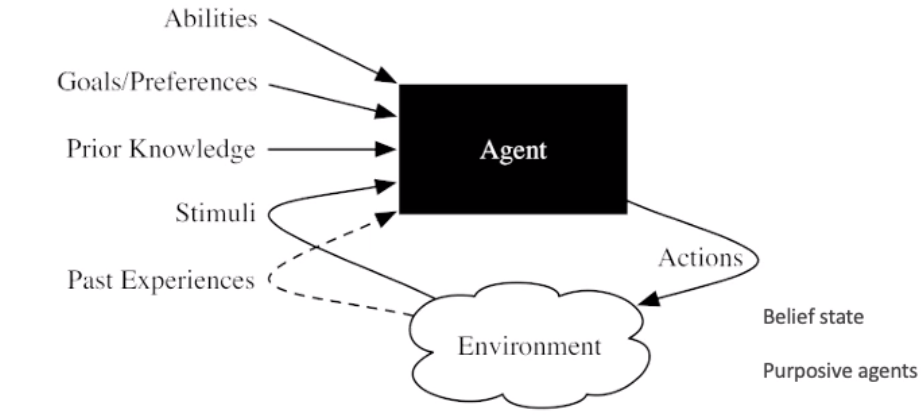
\includegraphics[scale=0.5]{1.png}
\end{center}
\paragraph{Design process}
\begin{list}{}{}
	\item design time computation, that goes into the design
	\item offline computation, that the agent can do before acting in the world (ex: specializing the model)
	\item online computation, done by the agent that is acting
\end{list}
Designing an intelligent agent that can adapt to complex environments and changing goals is a major challenge. Two strategies: simplify environments and build strong reasoning systems for these simple environments, or build simple agents for natural/complex environments simplifying the task.\\
\textbf{Steps} in the design process:
\begin{list}{}{}
	\item define the task in natural language, what need to be computed
	\item define what is a solution and its quality: optimal, satisfying, aproximately optimal, probable\ldots
	\item formal representation for the task, choosing how to represent knowledge for the task, including representations suitable for learning.
	\item compute an output
	\item interpret output as solution
\end{list}
\begin{center}
	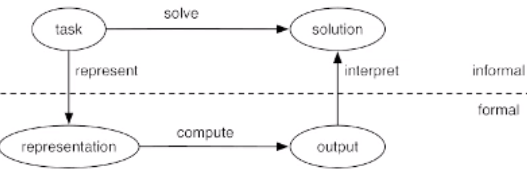
\includegraphics[scale=0.5]{2.png}
\end{center}
\paragraph{Levels of abstraction} A model of the world is a syumbolic rtepresentation of the beliefs of the agents. In is necessarily an abstraction: more abstract representations are simpler and human-readable but they may not be effective enough. Low level descriptions are more detailed and accurate but more complex too. Multiple level of abstractions are possibile (hierchical design). Two levels always present in the design: knowledge level (what the agent knows and its goals, not in terms of how we represent) and the symbol level (internal representation and reasoning system). \textbf{Modularity} extent to which a system/task can be decomposed \begin{list}{}{}
	\item flat: not modular
	\item modular: interacting modules that can be understood on their own
	\item hierarchical: modules are decomposed into simpler modules
\end{list}
\textbf{Planning horizon} how far ahead in time the agent plans \begin{list}{}{}
	\item non planning agent
	\item finite horizon planner: looks for a fixed amount of stages, greedy if only one step ahead
	\item indefinite horizon planner: finite but not predetermined number of stages
	\item infinite horizon planner: keeps planning forever (ex: stabilization module of a legged robot)
\end{list}
\textbf{Representation} concerns how the state of the world is described \begin{list}{}{}
	\item Atomic states
	\item feature-based representation: set of propositions that are true or false (PROP, CSP, most ML)
	\item individuals and relations, or relational representation
\end{list}
\textbf{Computational limits} that determines whether an agent has \begin{list}{}{}
	\item perfect rationality, reasons about the best actions without constraints
	\item bounded rationality, decides on the best action that it can find given its limits
\end{list}
An anytime algorithm is an algorithm where the solution improves with time.\\
\textbf{Learning dimensions} determines whether \begin{list}{}{}
	\item knowledge is given in advance, or
	\item knowledge is learned (from data or past experience)
\end{list}
Learning typically means finding the best model th %TODO
\textbf{Uncertainty}, which can be \begin{list}{}{}
	\item in sensing (fully/partially observable states)
	\item about the effects of the actions (deterministic/stochastic)
\end{list}
\textbf{Preference} dimension which considers thetehr the agent has
\begin{list}{}{}
	\item goal (achievemtn goal a proposition true in a final state, or mainentance goal, proposition true in all psobbile states)
	\item complex preferences, involving trade-offs among the desiderability of various\ldots %TODO
\end{list}
\textbf{Number of agents}\begin{list}{}{}
	\item single agent reasoning
	\item multi agent resoning
\end{list}
\textbf{Interaction} considers wheter the agent does:
\begin{list}{}{}
	\item offline reasoning or
	\item online reasoning
\end{list}
\paragraph{Agent Architectures} Agent interacts with an environment, receives informations with sensors and acts in the world with actuators. Robot: physical body. Program: software agent, digital environment.\\
Agent is made of body and controller, which receives percepts from the body and sends command to the body. A body includes sensors that converts stimuli into percepts and actautors that convert commands into actions.
\begin{center}
	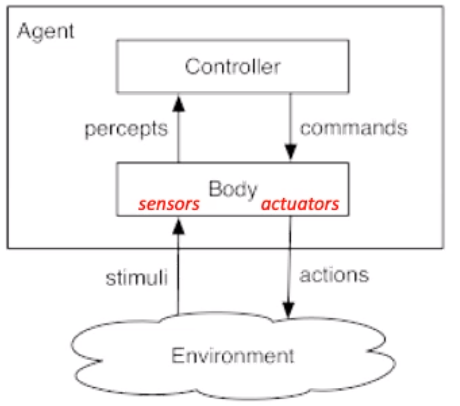
\includegraphics[scale=0.5]{3.png}
\end{center}
Bot sensors and %TODO
Agents act in time. $T$ is a set of time points, with start at 0, totally ordered, discrete and each $t$ has a next time $t+1$.\\
Percept trace/stream: function of time into percepts (past, present, future)\\
Command trace: a function of time into commands (past, present, future)\\
History at time $t$: percepts up to $t$ and commands up to $t-1$\\\\
Casual trasduction: a function from history to commands. Transduction comes from finite state transducers, where both new states and commands are emitted. Casual because only previous and current percepts and previous commands can be considered. A controller ideally implements a casual transduction.
\end{document}